% Options for packages loaded elsewhere
\PassOptionsToPackage{unicode}{hyperref}
\PassOptionsToPackage{hyphens}{url}
%
\documentclass[
]{article}
\usepackage{amsmath,amssymb}
\usepackage{lmodern}
\usepackage{iftex}
\ifPDFTeX
  \usepackage[T1]{fontenc}
  \usepackage[utf8]{inputenc}
  \usepackage{textcomp} % provide euro and other symbols
\else % if luatex or xetex
  \usepackage{unicode-math}
  \defaultfontfeatures{Scale=MatchLowercase}
  \defaultfontfeatures[\rmfamily]{Ligatures=TeX,Scale=1}
\fi
% Use upquote if available, for straight quotes in verbatim environments
\IfFileExists{upquote.sty}{\usepackage{upquote}}{}
\IfFileExists{microtype.sty}{% use microtype if available
  \usepackage[]{microtype}
  \UseMicrotypeSet[protrusion]{basicmath} % disable protrusion for tt fonts
}{}
\makeatletter
\@ifundefined{KOMAClassName}{% if non-KOMA class
  \IfFileExists{parskip.sty}{%
    \usepackage{parskip}
  }{% else
    \setlength{\parindent}{0pt}
    \setlength{\parskip}{6pt plus 2pt minus 1pt}}
}{% if KOMA class
  \KOMAoptions{parskip=half}}
\makeatother
\usepackage{xcolor}
\usepackage[margin=1in]{geometry}
\usepackage{color}
\usepackage{fancyvrb}
\newcommand{\VerbBar}{|}
\newcommand{\VERB}{\Verb[commandchars=\\\{\}]}
\DefineVerbatimEnvironment{Highlighting}{Verbatim}{commandchars=\\\{\}}
% Add ',fontsize=\small' for more characters per line
\usepackage{framed}
\definecolor{shadecolor}{RGB}{248,248,248}
\newenvironment{Shaded}{\begin{snugshade}}{\end{snugshade}}
\newcommand{\AlertTok}[1]{\textcolor[rgb]{0.94,0.16,0.16}{#1}}
\newcommand{\AnnotationTok}[1]{\textcolor[rgb]{0.56,0.35,0.01}{\textbf{\textit{#1}}}}
\newcommand{\AttributeTok}[1]{\textcolor[rgb]{0.77,0.63,0.00}{#1}}
\newcommand{\BaseNTok}[1]{\textcolor[rgb]{0.00,0.00,0.81}{#1}}
\newcommand{\BuiltInTok}[1]{#1}
\newcommand{\CharTok}[1]{\textcolor[rgb]{0.31,0.60,0.02}{#1}}
\newcommand{\CommentTok}[1]{\textcolor[rgb]{0.56,0.35,0.01}{\textit{#1}}}
\newcommand{\CommentVarTok}[1]{\textcolor[rgb]{0.56,0.35,0.01}{\textbf{\textit{#1}}}}
\newcommand{\ConstantTok}[1]{\textcolor[rgb]{0.00,0.00,0.00}{#1}}
\newcommand{\ControlFlowTok}[1]{\textcolor[rgb]{0.13,0.29,0.53}{\textbf{#1}}}
\newcommand{\DataTypeTok}[1]{\textcolor[rgb]{0.13,0.29,0.53}{#1}}
\newcommand{\DecValTok}[1]{\textcolor[rgb]{0.00,0.00,0.81}{#1}}
\newcommand{\DocumentationTok}[1]{\textcolor[rgb]{0.56,0.35,0.01}{\textbf{\textit{#1}}}}
\newcommand{\ErrorTok}[1]{\textcolor[rgb]{0.64,0.00,0.00}{\textbf{#1}}}
\newcommand{\ExtensionTok}[1]{#1}
\newcommand{\FloatTok}[1]{\textcolor[rgb]{0.00,0.00,0.81}{#1}}
\newcommand{\FunctionTok}[1]{\textcolor[rgb]{0.00,0.00,0.00}{#1}}
\newcommand{\ImportTok}[1]{#1}
\newcommand{\InformationTok}[1]{\textcolor[rgb]{0.56,0.35,0.01}{\textbf{\textit{#1}}}}
\newcommand{\KeywordTok}[1]{\textcolor[rgb]{0.13,0.29,0.53}{\textbf{#1}}}
\newcommand{\NormalTok}[1]{#1}
\newcommand{\OperatorTok}[1]{\textcolor[rgb]{0.81,0.36,0.00}{\textbf{#1}}}
\newcommand{\OtherTok}[1]{\textcolor[rgb]{0.56,0.35,0.01}{#1}}
\newcommand{\PreprocessorTok}[1]{\textcolor[rgb]{0.56,0.35,0.01}{\textit{#1}}}
\newcommand{\RegionMarkerTok}[1]{#1}
\newcommand{\SpecialCharTok}[1]{\textcolor[rgb]{0.00,0.00,0.00}{#1}}
\newcommand{\SpecialStringTok}[1]{\textcolor[rgb]{0.31,0.60,0.02}{#1}}
\newcommand{\StringTok}[1]{\textcolor[rgb]{0.31,0.60,0.02}{#1}}
\newcommand{\VariableTok}[1]{\textcolor[rgb]{0.00,0.00,0.00}{#1}}
\newcommand{\VerbatimStringTok}[1]{\textcolor[rgb]{0.31,0.60,0.02}{#1}}
\newcommand{\WarningTok}[1]{\textcolor[rgb]{0.56,0.35,0.01}{\textbf{\textit{#1}}}}
\usepackage{graphicx}
\makeatletter
\def\maxwidth{\ifdim\Gin@nat@width>\linewidth\linewidth\else\Gin@nat@width\fi}
\def\maxheight{\ifdim\Gin@nat@height>\textheight\textheight\else\Gin@nat@height\fi}
\makeatother
% Scale images if necessary, so that they will not overflow the page
% margins by default, and it is still possible to overwrite the defaults
% using explicit options in \includegraphics[width, height, ...]{}
\setkeys{Gin}{width=\maxwidth,height=\maxheight,keepaspectratio}
% Set default figure placement to htbp
\makeatletter
\def\fps@figure{htbp}
\makeatother
\setlength{\emergencystretch}{3em} % prevent overfull lines
\providecommand{\tightlist}{%
  \setlength{\itemsep}{0pt}\setlength{\parskip}{0pt}}
\setcounter{secnumdepth}{-\maxdimen} % remove section numbering
\ifLuaTeX
  \usepackage{selnolig}  % disable illegal ligatures
\fi
\IfFileExists{bookmark.sty}{\usepackage{bookmark}}{\usepackage{hyperref}}
\IfFileExists{xurl.sty}{\usepackage{xurl}}{} % add URL line breaks if available
\urlstyle{same} % disable monospaced font for URLs
\hypersetup{
  pdftitle={Earthquakes},
  pdfauthor={Samuel Richards},
  hidelinks,
  pdfcreator={LaTeX via pandoc}}

\title{Earthquakes}
\author{Samuel Richards}
\date{2023-03-22}

\begin{document}
\maketitle

Data was queried using USGS Earthquake Catalog:
\url{https://earthquake.usgs.gov/earthquakes/search/} to select all
recorded earthquakes of magnitude 4.5 and above with the following query
parameters:

\begin{itemize}
\tightlist
\item
  latitude 35.4 - 41.2
\item
  longitude 137.5 - 145.2
\item
  Timeframe(UTC): 2011-03-11 00:00:00 - 1965-01-01 00:00:00
\end{itemize}

The data was stored locally in a .csv file named \texttt{earthquakes}.

The organization also has an package called \texttt{rcomcat} to query
data directly into \texttt{R}, but its version was not compatible at the
time of this thesis.

\begin{Shaded}
\begin{Highlighting}[]
\CommentTok{\#read the data and create a new variable to be able to select annual timepoints while preserving the original timestamp}
\NormalTok{eq }\OtherTok{\textless{}{-}} \FunctionTok{read.csv}\NormalTok{(}\StringTok{"data/earthquakes.csv"}\NormalTok{) }\SpecialCharTok{\%\textgreater{}\%} 
  \FunctionTok{mutate}\NormalTok{(}\AttributeTok{timestamp =} \FunctionTok{ymd\_hms}\NormalTok{(time)) }\SpecialCharTok{\%\textgreater{}\%} 
  \FunctionTok{arrange}\NormalTok{(timestamp) }\SpecialCharTok{\%\textgreater{}\%} 
  \FunctionTok{mutate}\NormalTok{(}\AttributeTok{year =} \FunctionTok{year}\NormalTok{(timestamp))}


\CommentTok{\#subsets the data to include only the highest magnitude earthquake for each year (plus the most recent before the big one)}
\NormalTok{yearly }\OtherTok{\textless{}{-}}\NormalTok{ eq }\SpecialCharTok{\%\textgreater{}\%} \FunctionTok{group\_by}\NormalTok{(year) }\SpecialCharTok{\%\textgreater{}\%} 
  \FunctionTok{slice\_max}\NormalTok{(mag) }\SpecialCharTok{\%\textgreater{}\%} 
  \FunctionTok{distinct}\NormalTok{(year,}\AttributeTok{.keep\_all =}\NormalTok{ T) }\SpecialCharTok{\%\textgreater{}\%} 
  \FunctionTok{rbind}\NormalTok{(eq[}\DecValTok{3158}\NormalTok{,]) }\SpecialCharTok{\%\textgreater{}\%} 
  \FunctionTok{arrange}\NormalTok{(timestamp)}
\end{Highlighting}
\end{Shaded}

\hypertarget{plot-of-earthquakes}{%
\subsection{Plot of Earthquakes}\label{plot-of-earthquakes}}

The highest magnitude earthquake each year from 1965 - 2011

\hypertarget{data-preprocessing}{%
\subsection{Data Preprocessing}\label{data-preprocessing}}

\begin{Shaded}
\begin{Highlighting}[]
\CommentTok{\#Subset data to include observations from January 1, 1965 to the Greak Quake of March 11, 2011}
\NormalTok{eq }\OtherTok{\textless{}{-}}\NormalTok{ eq[}\FunctionTok{which}\NormalTok{(eq}\SpecialCharTok{$}\NormalTok{time }\SpecialCharTok{\textgreater{}=} \StringTok{"1965{-}01{-}26T23:47:37.120Z"} \SpecialCharTok{\&}\NormalTok{ eq}\SpecialCharTok{$}\NormalTok{time }\SpecialCharTok{\textless{}=} \StringTok{"2011{-}03{-}11T05:46:24.120Z}
\StringTok{"}\NormalTok{),]}

\CommentTok{\#If I want to subset by the same geographic area as the book}
\CommentTok{\#eq \textless{}{-} eq[which(eq$latitude \textgreater{} 37.72 \& eq$latitude \textless{} 38.82 \& eq$longitude \textgreater{} 141.87 \& eq$longitude \textless{} 142.87),]}

\CommentTok{\#Fine{-}tuning the geographic area of the model...}
\NormalTok{eq }\OtherTok{\textless{}{-}}\NormalTok{ eq[}\FunctionTok{which}\NormalTok{(eq}\SpecialCharTok{$}\NormalTok{latitude }\SpecialCharTok{\textgreater{}} \FloatTok{35.72} \SpecialCharTok{\&}\NormalTok{ eq}\SpecialCharTok{$}\NormalTok{latitude }\SpecialCharTok{\textless{}} \FloatTok{40.82} \SpecialCharTok{\&}\NormalTok{ eq}\SpecialCharTok{$}\NormalTok{longitude }\SpecialCharTok{\textgreater{}} \FloatTok{139.37} \SpecialCharTok{\&}\NormalTok{ eq}\SpecialCharTok{$}\NormalTok{longitude }\SpecialCharTok{\textless{}} \FloatTok{143.37}\NormalTok{),]}

\NormalTok{eq }\OtherTok{\textless{}{-}}\NormalTok{ eq[}\SpecialCharTok{{-}}\FunctionTok{as.numeric}\NormalTok{(}\FunctionTok{count}\NormalTok{(eq)),] }\CommentTok{\#to omit the 9.1}

\CommentTok{\#{-}{-}{-}data frame of magnitudes (rounded to .1) and relative frequencies}
\NormalTok{gg }\OtherTok{\textless{}{-}} \FunctionTok{data.frame}\NormalTok{(}\FunctionTok{table}\NormalTok{(}\FunctionTok{round}\NormalTok{(eq}\SpecialCharTok{$}\NormalTok{mag, }\DecValTok{1}\NormalTok{)) ) }\SpecialCharTok{\%\textgreater{}\%} 
  \FunctionTok{rename}\NormalTok{(}\AttributeTok{mag =}\NormalTok{ Var1,}
         \AttributeTok{freq =}\NormalTok{ Freq)}

\NormalTok{gg}\SpecialCharTok{$}\NormalTok{mag }\OtherTok{\textless{}{-}} \FunctionTok{as.numeric}\NormalTok{(}\FunctionTok{as.character}\NormalTok{(gg}\SpecialCharTok{$}\NormalTok{mag)) }\CommentTok{\#change to numeric rather than factors}

\NormalTok{gg}\SpecialCharTok{$}\NormalTok{freq }\OtherTok{\textless{}{-}}\NormalTok{ gg}\SpecialCharTok{$}\NormalTok{freq}\SpecialCharTok{/}\NormalTok{(}\DecValTok{2011{-}1965}\NormalTok{) }\CommentTok{\#AVERAGE annual frequencies over the 46{-}year span}


\CommentTok{\#creates a new variable representing the frequency of earthquakes of AT LEAST that magnitude}
\ControlFlowTok{for}\NormalTok{(i }\ControlFlowTok{in} \DecValTok{1}\SpecialCharTok{:}\FunctionTok{as.numeric}\NormalTok{(}\FunctionTok{count}\NormalTok{(gg)))\{}
\NormalTok{  gg}\SpecialCharTok{$}\NormalTok{freqc[i] }\OtherTok{\textless{}{-}} \FunctionTok{sum}\NormalTok{( gg}\SpecialCharTok{$}\NormalTok{freq[}\FunctionTok{c}\NormalTok{(i}\SpecialCharTok{:}\FunctionTok{as.numeric}\NormalTok{(}\FunctionTok{count}\NormalTok{(gg)))] )}
\NormalTok{\}}
\end{Highlighting}
\end{Shaded}

\hypertarget{frequency-of-earthquakes}{%
\subsection{Frequency of Earthquakes}\label{frequency-of-earthquakes}}

Relative to Magnitude

\begin{Shaded}
\begin{Highlighting}[]
\CommentTok{\#{-}{-}{-}frequencies of each magnitude}
\FunctionTok{ggplot}\NormalTok{(gg, }\FunctionTok{aes}\NormalTok{(}\AttributeTok{x =}\NormalTok{ mag, }\AttributeTok{y =}\NormalTok{ freqc)) }\SpecialCharTok{+}
  \FunctionTok{geom\_point}\NormalTok{(}\AttributeTok{size =} \DecValTok{4}\NormalTok{, }\AttributeTok{shape =} \DecValTok{17}\NormalTok{ ) }\SpecialCharTok{+}
    \FunctionTok{theme\_minimal}\NormalTok{() }\SpecialCharTok{+}
    \FunctionTok{labs}\NormalTok{(}\AttributeTok{x =} \StringTok{"Magnitude"}\NormalTok{,}
       \AttributeTok{y =} \StringTok{"Annual Frequency of At Least this Magnitude"}\NormalTok{,}
       \AttributeTok{title =} \StringTok{"Annual Earthquake Frequency near Tohoku, Japan"}\NormalTok{ ) }\SpecialCharTok{+}
  \FunctionTok{ylim}\NormalTok{(}\DecValTok{0}\NormalTok{,}\DecValTok{50}\NormalTok{)}
\end{Highlighting}
\end{Shaded}

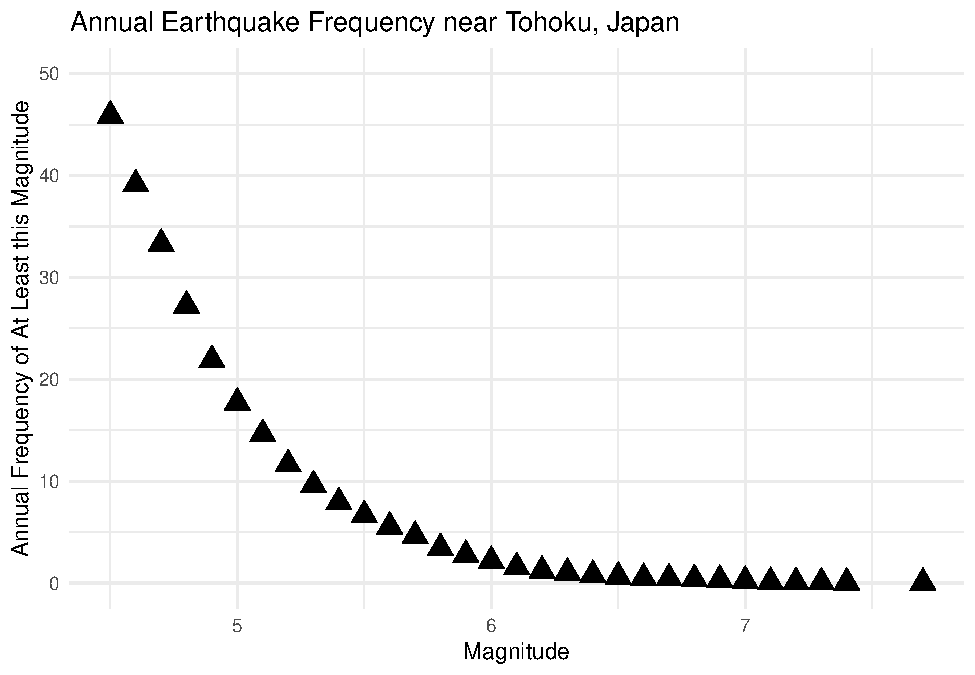
\includegraphics{earthquakes_files/figure-latex/unnamed-chunk-4-1.pdf}

\begin{Shaded}
\begin{Highlighting}[]
\CommentTok{\#{-}{-}{-}frequencies on the logarithmic scale}
\FunctionTok{ggplot}\NormalTok{(gg, }\FunctionTok{aes}\NormalTok{(}\AttributeTok{x =}\NormalTok{ mag, }\AttributeTok{y =}\NormalTok{ freqc)) }\SpecialCharTok{+}
  \FunctionTok{geom\_point}\NormalTok{(}\AttributeTok{size =} \DecValTok{4}\NormalTok{, }\AttributeTok{shape =} \DecValTok{17}\NormalTok{ ) }\SpecialCharTok{+}
  \FunctionTok{theme\_minimal}\NormalTok{() }\SpecialCharTok{+}
  \FunctionTok{scale\_y\_log10}\NormalTok{(}\AttributeTok{limits =} \FunctionTok{c}\NormalTok{(.}\DecValTok{001}\NormalTok{,}\DecValTok{100}\NormalTok{)) }\SpecialCharTok{+}
  \FunctionTok{scale\_x\_log10}\NormalTok{(}\AttributeTok{limits =} \FunctionTok{c}\NormalTok{(}\FloatTok{4.5}\NormalTok{,}\DecValTok{10}\NormalTok{)) }\SpecialCharTok{+}
  \FunctionTok{labs}\NormalTok{(}\AttributeTok{x =} \StringTok{"Magnitude"}\NormalTok{,}
       \AttributeTok{y =} \StringTok{"Annual Frequency of At Least this Magnitude"}\NormalTok{,}
       \AttributeTok{title =} \StringTok{"Annual Earthquake Frequency near Tohoku, Japan {-} Logarithmic Scale"}\NormalTok{ ) }\SpecialCharTok{+}
  \FunctionTok{stat\_smooth}\NormalTok{(}\AttributeTok{method =}\NormalTok{ lm,}
              \AttributeTok{formula =}\NormalTok{ y }\SpecialCharTok{\textasciitilde{}} \FunctionTok{poly}\NormalTok{(x,}\DecValTok{1}\NormalTok{),}
              \AttributeTok{fullrange =}\NormalTok{ T)}
\end{Highlighting}
\end{Shaded}

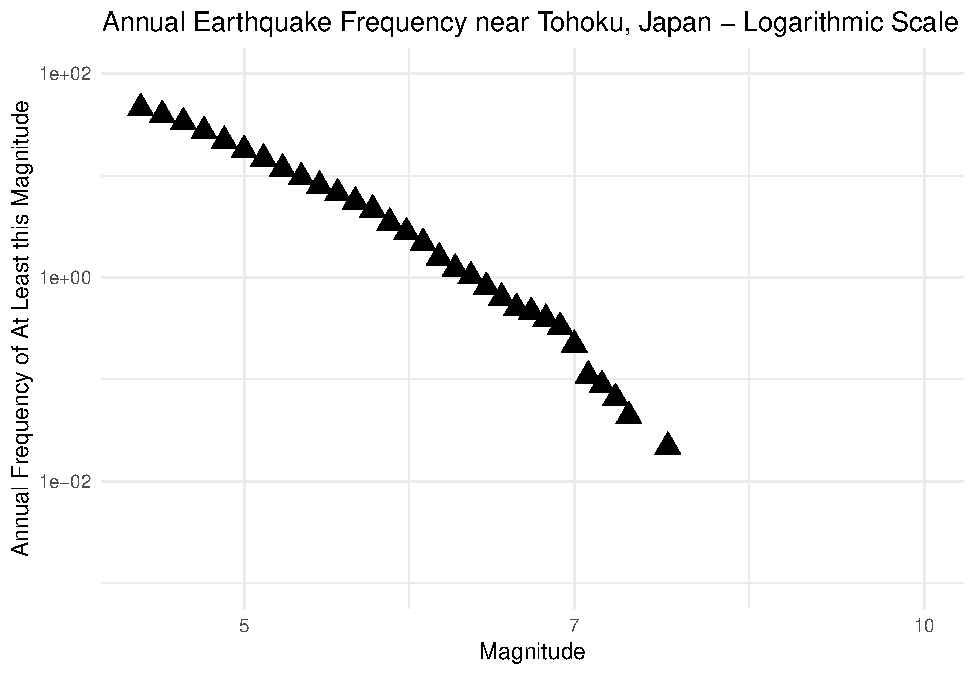
\includegraphics{earthquakes_files/figure-latex/unnamed-chunk-4-2.pdf}

\begin{Shaded}
\begin{Highlighting}[]
\NormalTok{earthquakes }\OtherTok{\textless{}{-}}\NormalTok{ gg}
\end{Highlighting}
\end{Shaded}

\hypertarget{linear-models-of-the-data}{%
\subsection{Linear models of the data}\label{linear-models-of-the-data}}

After log transformation of the data, a linear model is fit using
\texttt{R}.

\begin{Shaded}
\begin{Highlighting}[]
\CommentTok{\#{-}{-}{-}modeling{-}{-}{-}}
\NormalTok{earthquakes\_log }\OtherTok{\textless{}{-}}\NormalTok{ earthquakes }\SpecialCharTok{\%\textgreater{}\%} \FunctionTok{mutate}\NormalTok{(}\AttributeTok{freqc =} \FunctionTok{log10}\NormalTok{(freqc)) }\CommentTok{\#transforming to the log scale}

\NormalTok{linear }\OtherTok{\textless{}{-}} \FunctionTok{lm}\NormalTok{(}\AttributeTok{data =}\NormalTok{ earthquakes\_log, }\AttributeTok{formula =}\NormalTok{ freqc }\SpecialCharTok{\textasciitilde{}}\NormalTok{ mag)}

\FunctionTok{summary}\NormalTok{(linear)}
\end{Highlighting}
\end{Shaded}

\begin{verbatim}
## 
## Call:
## lm(formula = freqc ~ mag, data = earthquakes_log)
## 
## Residuals:
##      Min       1Q   Median       3Q      Max 
## -0.19955 -0.06120  0.02396  0.06852  0.16566 
## 
## Coefficients:
##             Estimate Std. Error t value Pr(>|t|)    
## (Intercept)  6.38365    0.11513   55.45   <2e-16 ***
## mag         -1.01971    0.01895  -53.80   <2e-16 ***
## ---
## Signif. codes:  0 '***' 0.001 '**' 0.01 '*' 0.05 '.' 0.1 ' ' 1
## 
## Residual standard error: 0.0956 on 29 degrees of freedom
## Multiple R-squared:  0.9901, Adjusted R-squared:  0.9897 
## F-statistic:  2894 on 1 and 29 DF,  p-value: < 2.2e-16
\end{verbatim}

\begin{Shaded}
\begin{Highlighting}[]
\NormalTok{p }\OtherTok{\textless{}{-}} \FunctionTok{predict}\NormalTok{(linear, }\AttributeTok{newdata =} \FunctionTok{data.frame}\NormalTok{(}\AttributeTok{mag =} \FloatTok{9.1}\NormalTok{))}

\CommentTok{\#{-}{-}{-}using caret yields the same prediction values but different coefficients from summary()???}
\CommentTok{\# fitControl \textless{}{-} trainControl(method = "cv", number = 10)}
\CommentTok{\# }
\CommentTok{\# b \textless{}{-} train(freqc \textasciitilde{} poly(mag,1), data = earthquakes\_log,}
\CommentTok{\#       method = "lm",}
\CommentTok{\#       preProc = c("center", "scale"),}
\CommentTok{\#       trControl = fitControl)}
\CommentTok{\# }
\CommentTok{\# summary(b)}
\CommentTok{\# }
\CommentTok{\# p \textless{}{-} predict(b, newdata = data.frame(mag = 9.1))}

\DecValTok{1}\SpecialCharTok{/}\DecValTok{10}\SpecialCharTok{\^{}}\NormalTok{p }\CommentTok{\#undo log transform for final result}
\end{Highlighting}
\end{Shaded}

\begin{verbatim}
##        1 
## 786.4653
\end{verbatim}

\begin{Shaded}
\begin{Highlighting}[]
\CommentTok{\#linear model with no polynomial terms predicts 0.001271512 {-} one every 786 years or so}
\CommentTok{\#model with second order polynomial predicts 0.0001756346  {-} one every 5694 years or so.}
\CommentTok{\#model with third order polynomial predicts 4.045112e{-}05  {-} one every 24721 years or so.}
\CommentTok{\#model with fourh order polynomial predicts 2.049643e{-}05   {-} one every 48789 years or so.}
\end{Highlighting}
\end{Shaded}

For completeness, this model shows that on average, for every 1.0
increase in magnitude, the lapsed time between earthquakes of \emph{at
least} that magnitude is expected to increase by \(1/10^{-1.01971}\) =
10.4642956 years.

For a magnitude 9.1 earthquake, the expected frequency would be one
every \(1/10^{6.38365-1.01971(9.1)}\) = \texttt{1/10\^{}p} years.

\begin{Shaded}
\begin{Highlighting}[]
\NormalTok{capacity }\OtherTok{\textless{}{-}} \DecValTok{1}\SpecialCharTok{:}\DecValTok{8}
\NormalTok{prediction }\OtherTok{\textless{}{-}} \ConstantTok{NULL}

\ControlFlowTok{for}\NormalTok{(i }\ControlFlowTok{in}\NormalTok{ capacity)\{}
\NormalTok{  linear }\OtherTok{\textless{}{-}} \FunctionTok{lm}\NormalTok{(}\AttributeTok{data =}\NormalTok{ earthquakes\_log, }\AttributeTok{formula =}\NormalTok{ freqc }\SpecialCharTok{\textasciitilde{}} \FunctionTok{poly}\NormalTok{(mag,i))}
\NormalTok{  p }\OtherTok{\textless{}{-}} \FunctionTok{predict}\NormalTok{(linear, }\AttributeTok{newdata =} \FunctionTok{data.frame}\NormalTok{(}\AttributeTok{mag =} \FloatTok{9.1}\NormalTok{))}
\NormalTok{  prediction[i] }\OtherTok{\textless{}{-}} \DecValTok{1}\SpecialCharTok{/}\DecValTok{10}\SpecialCharTok{\^{}}\NormalTok{p}
\NormalTok{\}}
\FunctionTok{data.frame}\NormalTok{(capacity,prediction)}
\end{Highlighting}
\end{Shaded}

\begin{verbatim}
##   capacity    prediction
## 1        1  7.864653e+02
## 2        2  5.693638e+03
## 3        3  2.472119e+04
## 4        4  4.878898e+04
## 5        5  4.513788e-01
## 6        6  1.522366e-33
## 7        7 8.608668e-153
## 8        8  6.102735e-40
\end{verbatim}

\end{document}
